\documentclass{standalone}
\usepackage{tikz}
\usetikzlibrary{patterns, positioning}


\begin{document}
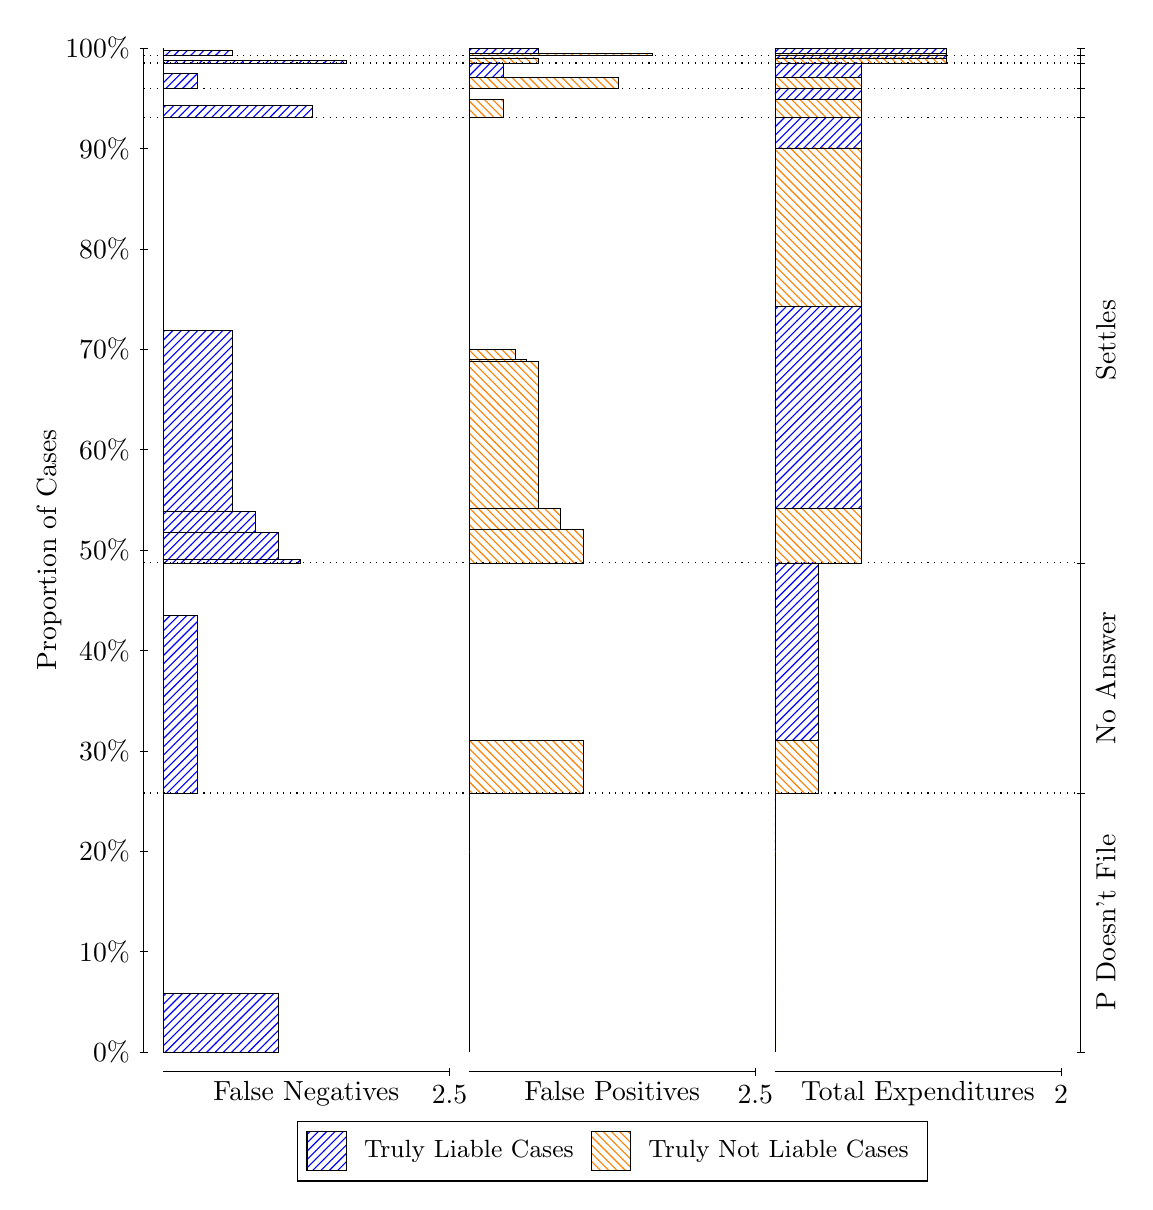
\begin{tikzpicture}
\draw[black, very thin] (1.5,1.75) -- (1.5,14.5);
\node[rotate=90, text=black, anchor=center] at (0.3, 8.125) {Proportion of Cases};
\draw[black, very thin] (1.45,1.75) -- (1.55,1.75);
\node[text=black, anchor=east] at (1.45, 1.75) {0\%};
\draw[black, very thin] (1.45,3.025) -- (1.55,3.025);
\node[text=black, anchor=east] at (1.45, 3.025) {10\%};
\draw[black, very thin] (1.45,4.3) -- (1.55,4.3);
\node[text=black, anchor=east] at (1.45, 4.3) {20\%};
\draw[black, very thin] (1.45,5.575) -- (1.55,5.575);
\node[text=black, anchor=east] at (1.45, 5.575) {30\%};
\draw[black, very thin] (1.45,6.85) -- (1.55,6.85);
\node[text=black, anchor=east] at (1.45, 6.85) {40\%};
\draw[black, very thin] (1.45,8.125) -- (1.55,8.125);
\node[text=black, anchor=east] at (1.45, 8.125) {50\%};
\draw[black, very thin] (1.45,9.4) -- (1.55,9.4);
\node[text=black, anchor=east] at (1.45, 9.4) {60\%};
\draw[black, very thin] (1.45,10.675) -- (1.55,10.675);
\node[text=black, anchor=east] at (1.45, 10.675) {70\%};
\draw[black, very thin] (1.45,11.95) -- (1.55,11.95);
\node[text=black, anchor=east] at (1.45, 11.95) {80\%};
\draw[black, very thin] (1.45,13.225) -- (1.55,13.225);
\node[text=black, anchor=east] at (1.45, 13.225) {90\%};
\draw[black, very thin] (1.45,14.5) -- (1.55,14.5);
\node[text=black, anchor=east] at (1.45, 14.5) {100\%};

\draw[black, very thin] (13.4,1.75) -- (13.4,14.5);
\draw[black, very thin] (13.35,1.75) -- (13.45,1.75);
\node[anchor=west] at (13.35, 1.75) {};
\draw[black, very thin] (13.35,5.0386) -- (13.45,5.0386);
\node[anchor=west] at (13.35, 5.0386) {};
\draw[black, very thin] (13.35,7.9621) -- (13.45,7.9621);
\node[anchor=west] at (13.35, 7.9621) {};
\draw[black, very thin] (13.35,13.621) -- (13.45,13.621);
\node[anchor=west] at (13.35, 13.621) {};
\draw[black, very thin] (13.35,13.991) -- (13.45,13.991);
\node[anchor=west] at (13.35, 13.991) {};
\draw[black, very thin] (13.35,14.31) -- (13.45,14.31);
\node[anchor=west] at (13.35, 14.31) {};
\draw[black, very thin] (13.35,14.404) -- (13.45,14.404);
\node[anchor=west] at (13.35, 14.404) {};
\draw[black, very thin] (13.35,14.5) -- (13.45,14.5);
\node[anchor=west] at (13.35, 14.5) {};

\draw[black, very thin, pattern color=blue, pattern=north east lines] (1.75,1.75) rectangle (3.2033,2.4912);
\draw[black, very thin, pattern color=orange, pattern=north west lines] (1.75,2.4912) rectangle (1.75,5.0386);
\draw[black, very thin, pattern color=blue, pattern=north east lines] (1.75,5.0386) rectangle (2.186,7.2938);
\draw[black, very thin, pattern color=orange, pattern=north west lines] (1.75,7.2938) rectangle (1.75,7.9621);
\draw[black, very thin, pattern color=blue, pattern=north east lines] (1.75,7.9621) rectangle (3.494,8.0019);
\draw[black, very thin, pattern color=blue, pattern=north east lines] (1.75,8.0019) rectangle (3.3487,8.0079);
\draw[black, very thin, pattern color=blue, pattern=north east lines] (1.75,8.0079) rectangle (3.2033,8.3504);
\draw[black, very thin, pattern color=blue, pattern=north east lines] (1.75,8.3504) rectangle (2.9127,8.6146);
\draw[black, very thin, pattern color=blue, pattern=north east lines] (1.75,8.6146) rectangle (2.622,10.914);
\draw[black, very thin, pattern color=orange, pattern=north west lines] (1.75,10.914) rectangle (1.75,13.621);
\draw[black, very thin, pattern color=blue, pattern=north east lines] (1.75,13.621) rectangle (3.6393,13.768);
\draw[black, very thin, pattern color=orange, pattern=north west lines] (1.75,13.768) rectangle (1.75,13.991);
\draw[black, very thin, pattern color=blue, pattern=north east lines] (1.75,13.991) rectangle (2.186,14.174);
\draw[black, very thin, pattern color=orange, pattern=north west lines] (1.75,14.174) rectangle (1.75,14.31);
\draw[black, very thin, pattern color=blue, pattern=north east lines] (1.75,14.31) rectangle (4.0753,14.339);
\draw[black, very thin, pattern color=orange, pattern=north west lines] (1.75,14.339) rectangle (1.75,14.404);
\draw[black, very thin, pattern color=blue, pattern=north east lines] (1.75,14.404) rectangle (2.622,14.47);
\draw[black, very thin, pattern color=orange, pattern=north west lines] (1.75,14.47) rectangle (1.75,14.5);
\draw[black, very thin, pattern color=orange, pattern=north west lines] (5.6333,1.75) rectangle (5.6333,4.2974);
\draw[black, very thin, pattern color=blue, pattern=north east lines] (5.6333,4.2974) rectangle (5.6333,5.0386);
\draw[black, very thin, pattern color=orange, pattern=north west lines] (5.6333,5.0386) rectangle (7.0867,5.7068);
\draw[black, very thin, pattern color=blue, pattern=north east lines] (5.6333,5.7068) rectangle (5.6333,7.9621);
\draw[black, very thin, pattern color=orange, pattern=north west lines] (5.6333,7.9621) rectangle (7.0867,8.386);
\draw[black, very thin, pattern color=orange, pattern=north west lines] (5.6333,8.386) rectangle (6.796,8.6503);
\draw[black, very thin, pattern color=orange, pattern=north west lines] (5.6333,8.6503) rectangle (6.5053,10.524);
\draw[black, very thin, pattern color=orange, pattern=north west lines] (5.6333,10.524) rectangle (6.36,10.541);
\draw[black, very thin, pattern color=orange, pattern=north west lines] (5.6333,10.541) rectangle (6.2147,10.669);
\draw[black, very thin, pattern color=blue, pattern=north east lines] (5.6333,10.669) rectangle (5.6333,13.621);
\draw[black, very thin, pattern color=orange, pattern=north west lines] (5.6333,13.621) rectangle (6.0693,13.844);
\draw[black, very thin, pattern color=blue, pattern=north east lines] (5.6333,13.844) rectangle (5.6333,13.991);
\draw[black, very thin, pattern color=orange, pattern=north west lines] (5.6333,13.991) rectangle (7.5227,14.126);
\draw[black, very thin, pattern color=blue, pattern=north east lines] (5.6333,14.126) rectangle (6.0693,14.31);
\draw[black, very thin, pattern color=orange, pattern=north west lines] (5.6333,14.31) rectangle (6.5053,14.375);
\draw[black, very thin, pattern color=blue, pattern=north east lines] (5.6333,14.375) rectangle (5.6333,14.404);
\draw[black, very thin, pattern color=orange, pattern=north west lines] (5.6333,14.404) rectangle (7.9587,14.434);
\draw[black, very thin, pattern color=blue, pattern=north east lines] (5.6333,14.434) rectangle (6.5053,14.5);
\draw[black, very thin, pattern color=orange, pattern=north west lines] (9.5167,1.75) rectangle (9.5167,4.2974);
\draw[black, very thin, pattern color=blue, pattern=north east lines] (9.5167,4.2974) rectangle (9.5167,5.0386);
\draw[black, very thin, pattern color=orange, pattern=north west lines] (9.5167,5.0386) rectangle (10.062,5.7068);
\draw[black, very thin, pattern color=blue, pattern=north east lines] (9.5167,5.7068) rectangle (10.062,7.9621);
\draw[black, very thin, pattern color=orange, pattern=north west lines] (9.5167,7.9621) rectangle (10.607,8.6503);
\draw[black, very thin, pattern color=blue, pattern=north east lines] (9.5167,8.6503) rectangle (10.607,11.214);
\draw[black, very thin, pattern color=orange, pattern=north west lines] (9.5167,11.214) rectangle (10.607,13.233);
\draw[black, very thin, pattern color=blue, pattern=north east lines] (9.5167,13.233) rectangle (10.607,13.621);
\draw[black, very thin, pattern color=orange, pattern=north west lines] (9.5167,13.621) rectangle (10.607,13.844);
\draw[black, very thin, pattern color=blue, pattern=north east lines] (9.5167,13.844) rectangle (10.607,13.991);
\draw[black, very thin, pattern color=orange, pattern=north west lines] (9.5167,13.991) rectangle (10.607,14.126);
\draw[black, very thin, pattern color=blue, pattern=north east lines] (9.5167,14.126) rectangle (10.607,14.31);
\draw[black, very thin, pattern color=orange, pattern=north west lines] (9.5167,14.31) rectangle (11.697,14.375);
\draw[black, very thin, pattern color=blue, pattern=north east lines] (9.5167,14.375) rectangle (11.697,14.404);
\draw[black, very thin, pattern color=orange, pattern=north west lines] (9.5167,14.404) rectangle (11.697,14.434);
\draw[black, very thin, pattern color=blue, pattern=north east lines] (9.5167,14.434) rectangle (11.697,14.5);
\draw[black, dotted] (1.5,5.0386) -- (13.4,5.0386);
\draw[black, dotted] (1.5,7.9621) -- (13.4,7.9621);
\draw[black, dotted] (1.5,13.621) -- (13.4,13.621);
\draw[black, dotted] (1.5,13.991) -- (13.4,13.991);
\draw[black, dotted] (1.5,14.31) -- (13.4,14.31);
\draw[black, dotted] (1.5,14.404) -- (13.4,14.404);
\draw[black, very thin] (1.75,1.5) -- (5.3833,1.5);
\node[text=black, anchor=north] at (3.5667, 1.5) {False Negatives};
\draw[black, very thin] (5.3833,1.45) -- (5.3833,1.55);
\node[text=black, anchor=north] at (5.3833, 1.45) {2.5};

\draw[black, very thin] (5.6333,1.5) -- (9.2667,1.5);
\node[text=black, anchor=north] at (7.45, 1.5) {False Positives};
\draw[black, very thin] (9.2667,1.45) -- (9.2667,1.55);
\node[text=black, anchor=north] at (9.2667, 1.45) {2.5};

\draw[black, very thin] (9.5167,1.5) -- (13.15,1.5);
\node[text=black, anchor=north] at (11.333, 1.5) {Total Expenditures};
\draw[black, very thin] (13.15,1.45) -- (13.15,1.55);
\node[text=black, anchor=north] at (13.15, 1.45) {2};

\node[text=black, centered, rotate=90] at (13.72, 3.3943) {P Doesn't File};
\node[text=black, centered, rotate=90] at (13.72, 6.5003) {No Answer};
\node[text=black, centered, rotate=90] at (13.72, 10.792) {Settles};





\draw (7.449999999999999,1.5) node[draw=none] (baseCoordinate) {};
\begin{scope}[align=center]
        \matrix[scale=0.5, draw=black, below=0.5cm of baseCoordinate, nodes={draw}, column sep=0.1cm]{
            \node[rectangle, draw, minimum width=0.5cm, minimum height=0.5cm, pattern color=blue, pattern=north east lines] {}; &
            \node[draw=none, font=\small, text=black] (B) {Truly Liable Cases}; &
            \node[rectangle, draw, minimum width=0.5cm, minimum height=0.5cm, pattern color=orange, pattern=north west lines] {}; &
            \node[draw=none, font=\small, text=black] (B) {Truly Not Liable Cases}; \\
            };
\end{scope}

\end{tikzpicture}
\end{document}